\providecommand{\main}{../../../..}
\documentclass[\main/dresen_thesis.tex]{subfiles}
\begin{document}
  \label{sec:monolayers:nanoparticle:saxs}

  \paragraphNewLine{Small-Angle Scattering}
    A macroscopic area of the samples is quantitatively evaluated to determine the average nuclear and magnetic structure of the diluted nanoparticles in dispersion using small-angle X-ray and (polarized) neutron scattering in \reffig{fig:monolayers:nanoparticle:sas:AcOlCoFeC}.

    The comparison between the Ol-CoFe-C and Ac-CoFe-C small-angle scattering data shows on a qualitative level that the nanocubes synthesized following the oleate route have a smaller size distribution and higher homogeneous sample quality as more oscillations are visible with more pronounced minima, confirming the result observed from TEM.
    However, it also shows that Ol-CoFe-C is only weakly magnetic whereas the particles in Ac-CoFe-C have a stronger magnetic moment, which is visible in the greater splitting of $I(+)$ and $I(-)$ in SANSPOL.
    
    \begin{figure}[tb]
      \centering
      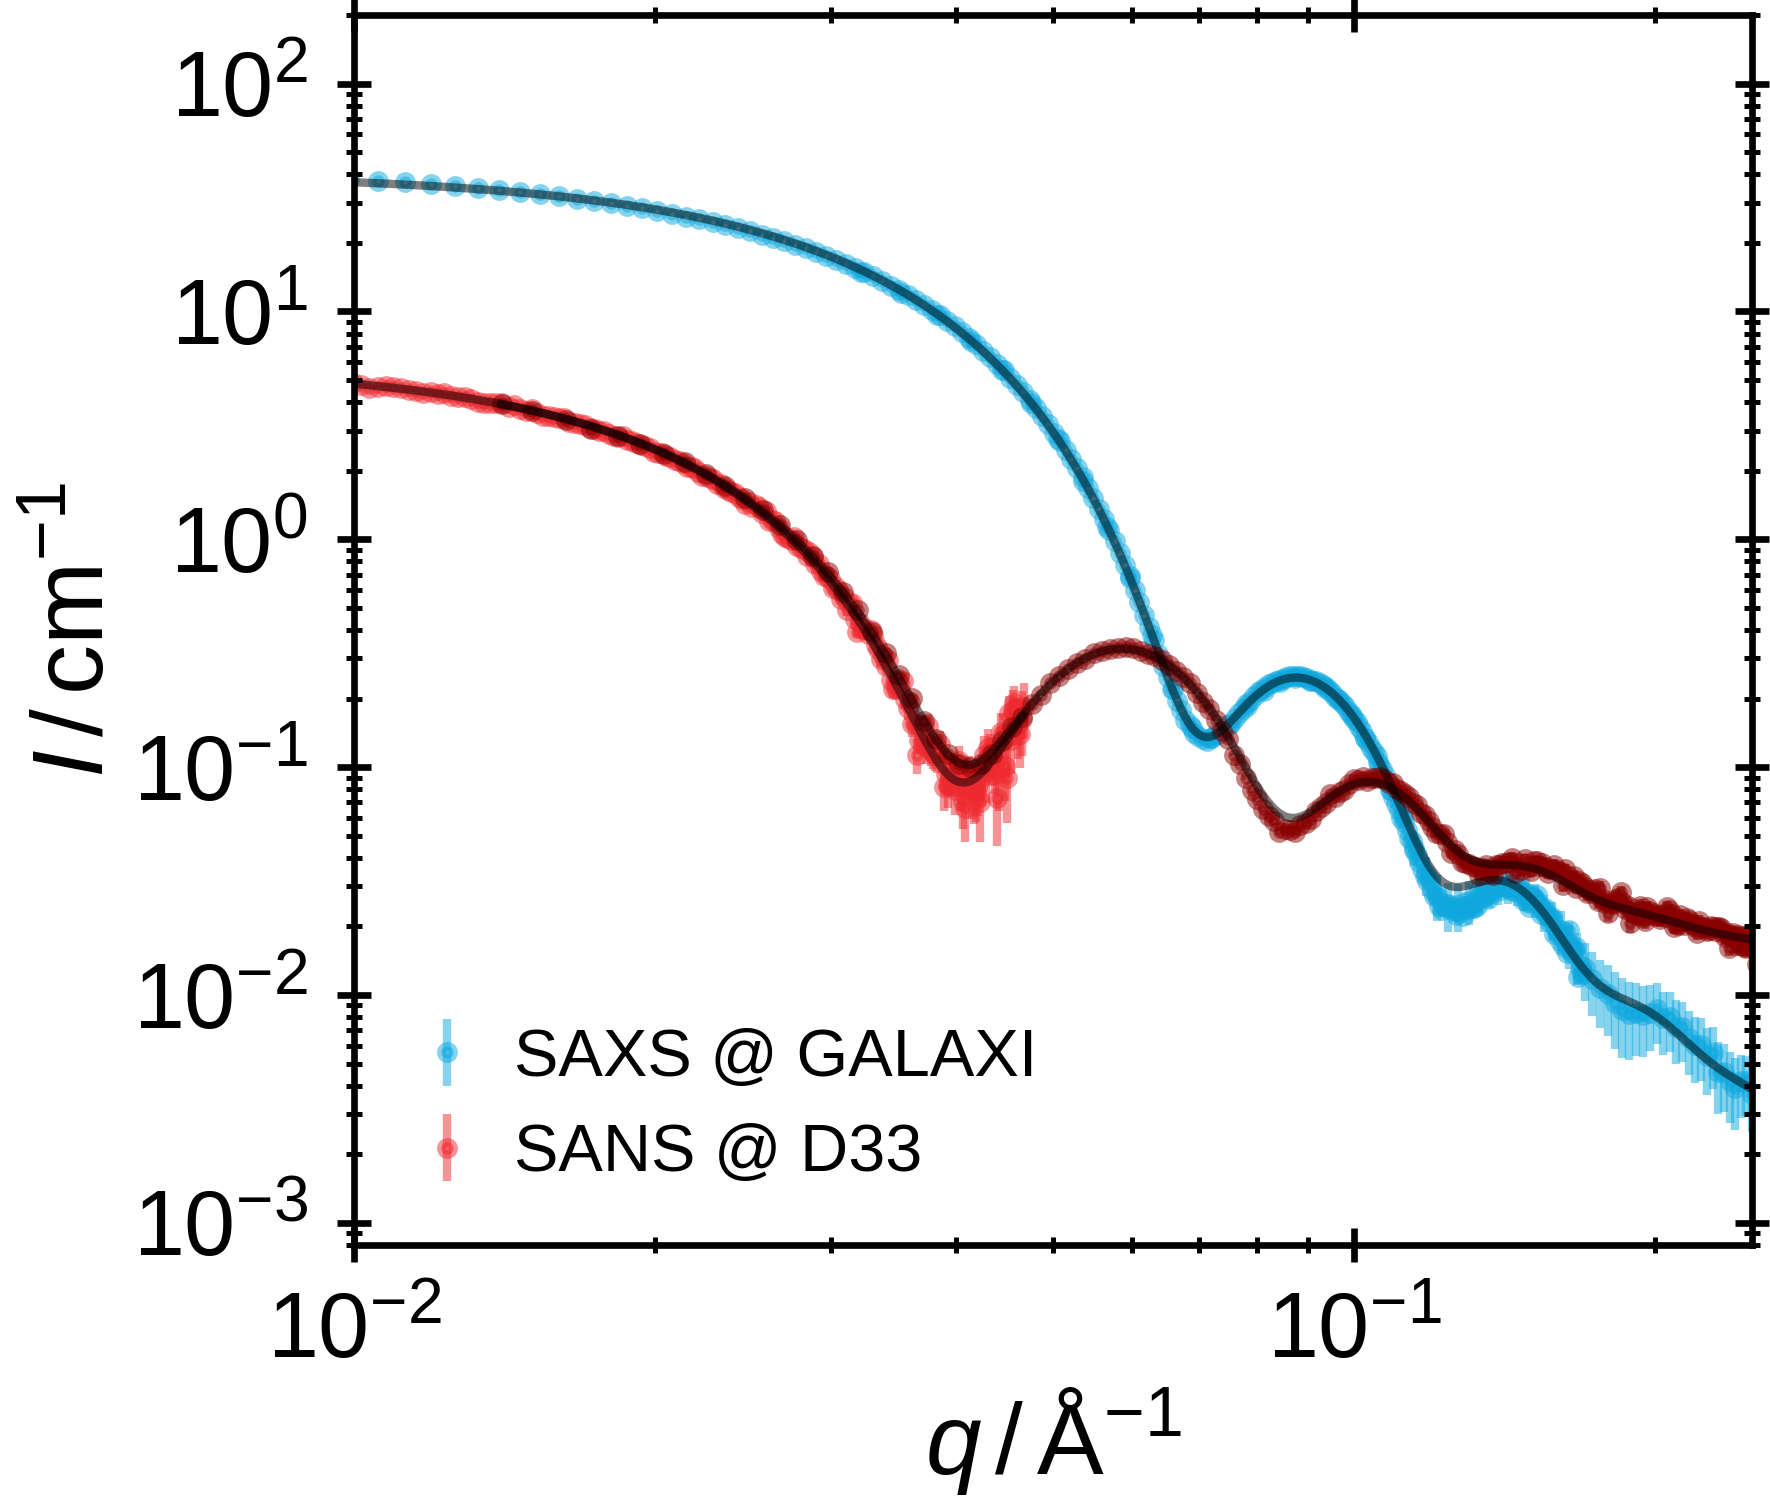
\includegraphics{monolayers_SAS_Ol_CoFe_C_SASFit}
      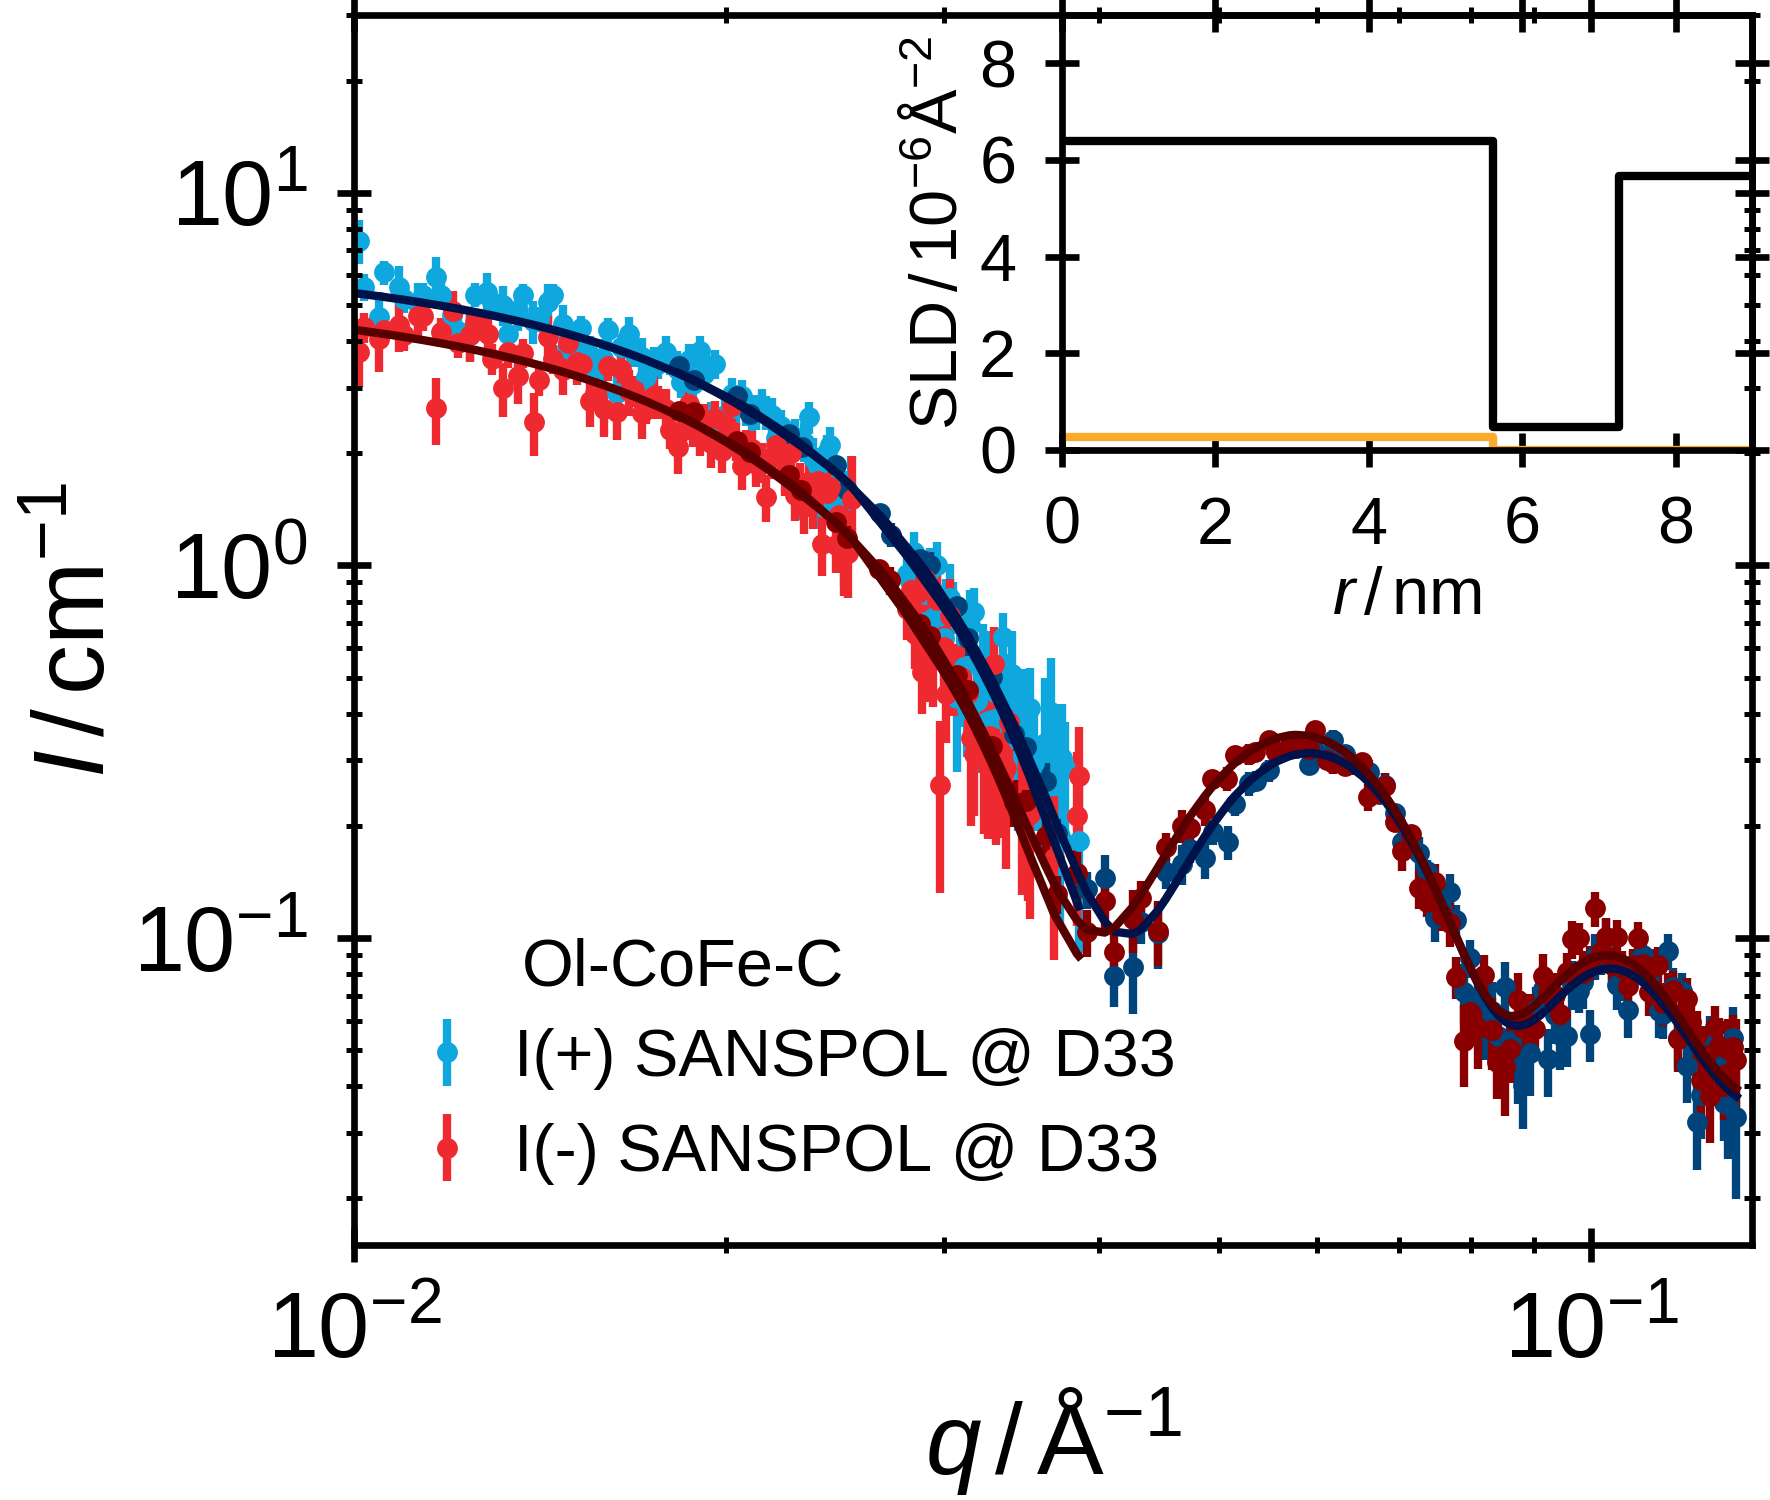
\includegraphics{monolayers_SAS_Ol_CoFe_C_SANSPOLFit}
      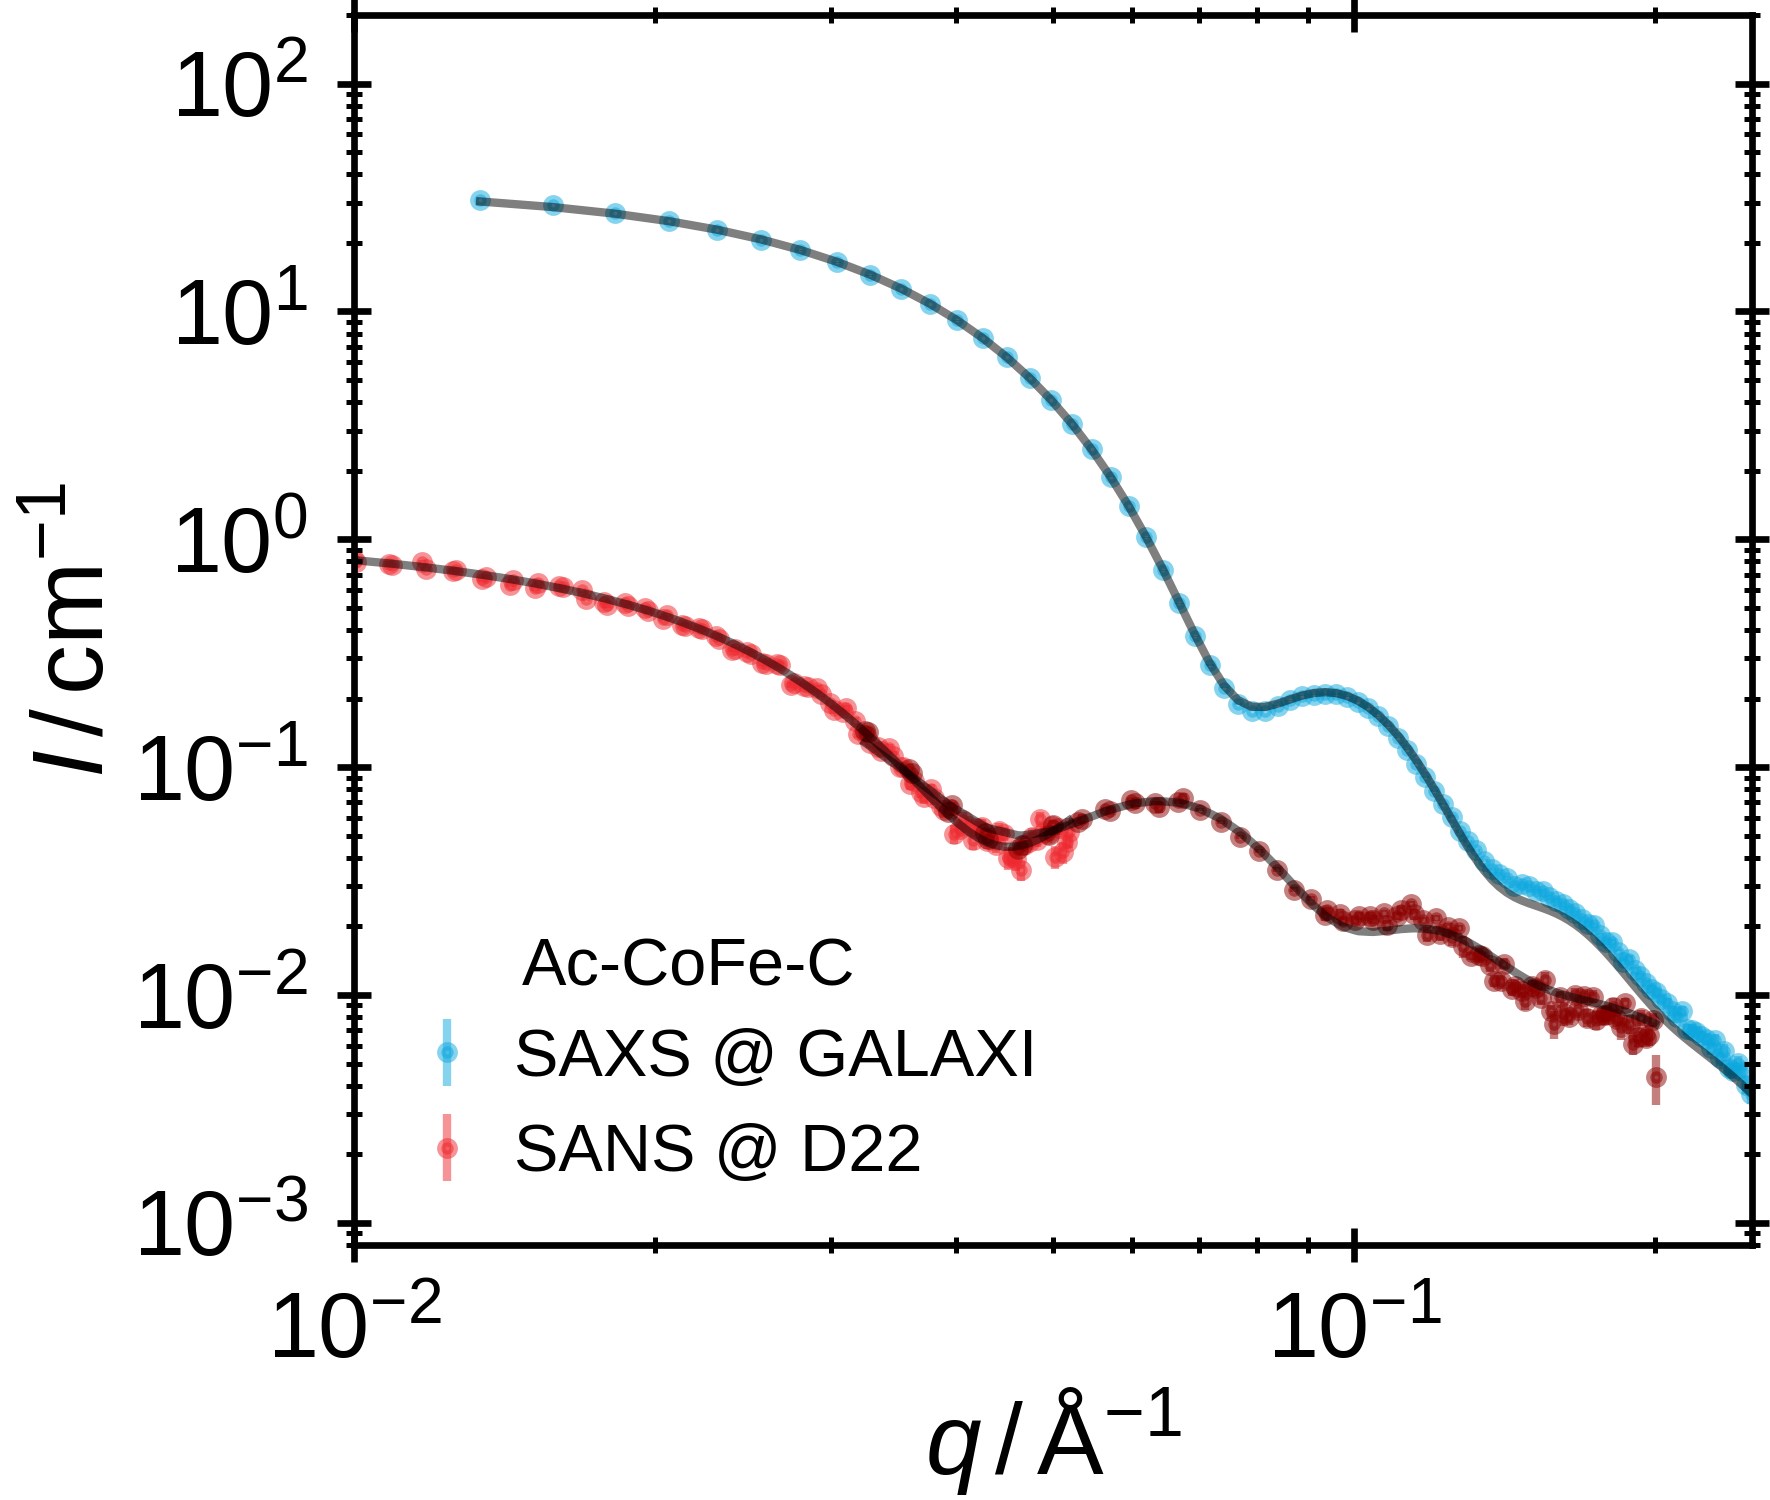
\includegraphics{monolayers_SAS_Ac_CoFe_C_SASFit}
      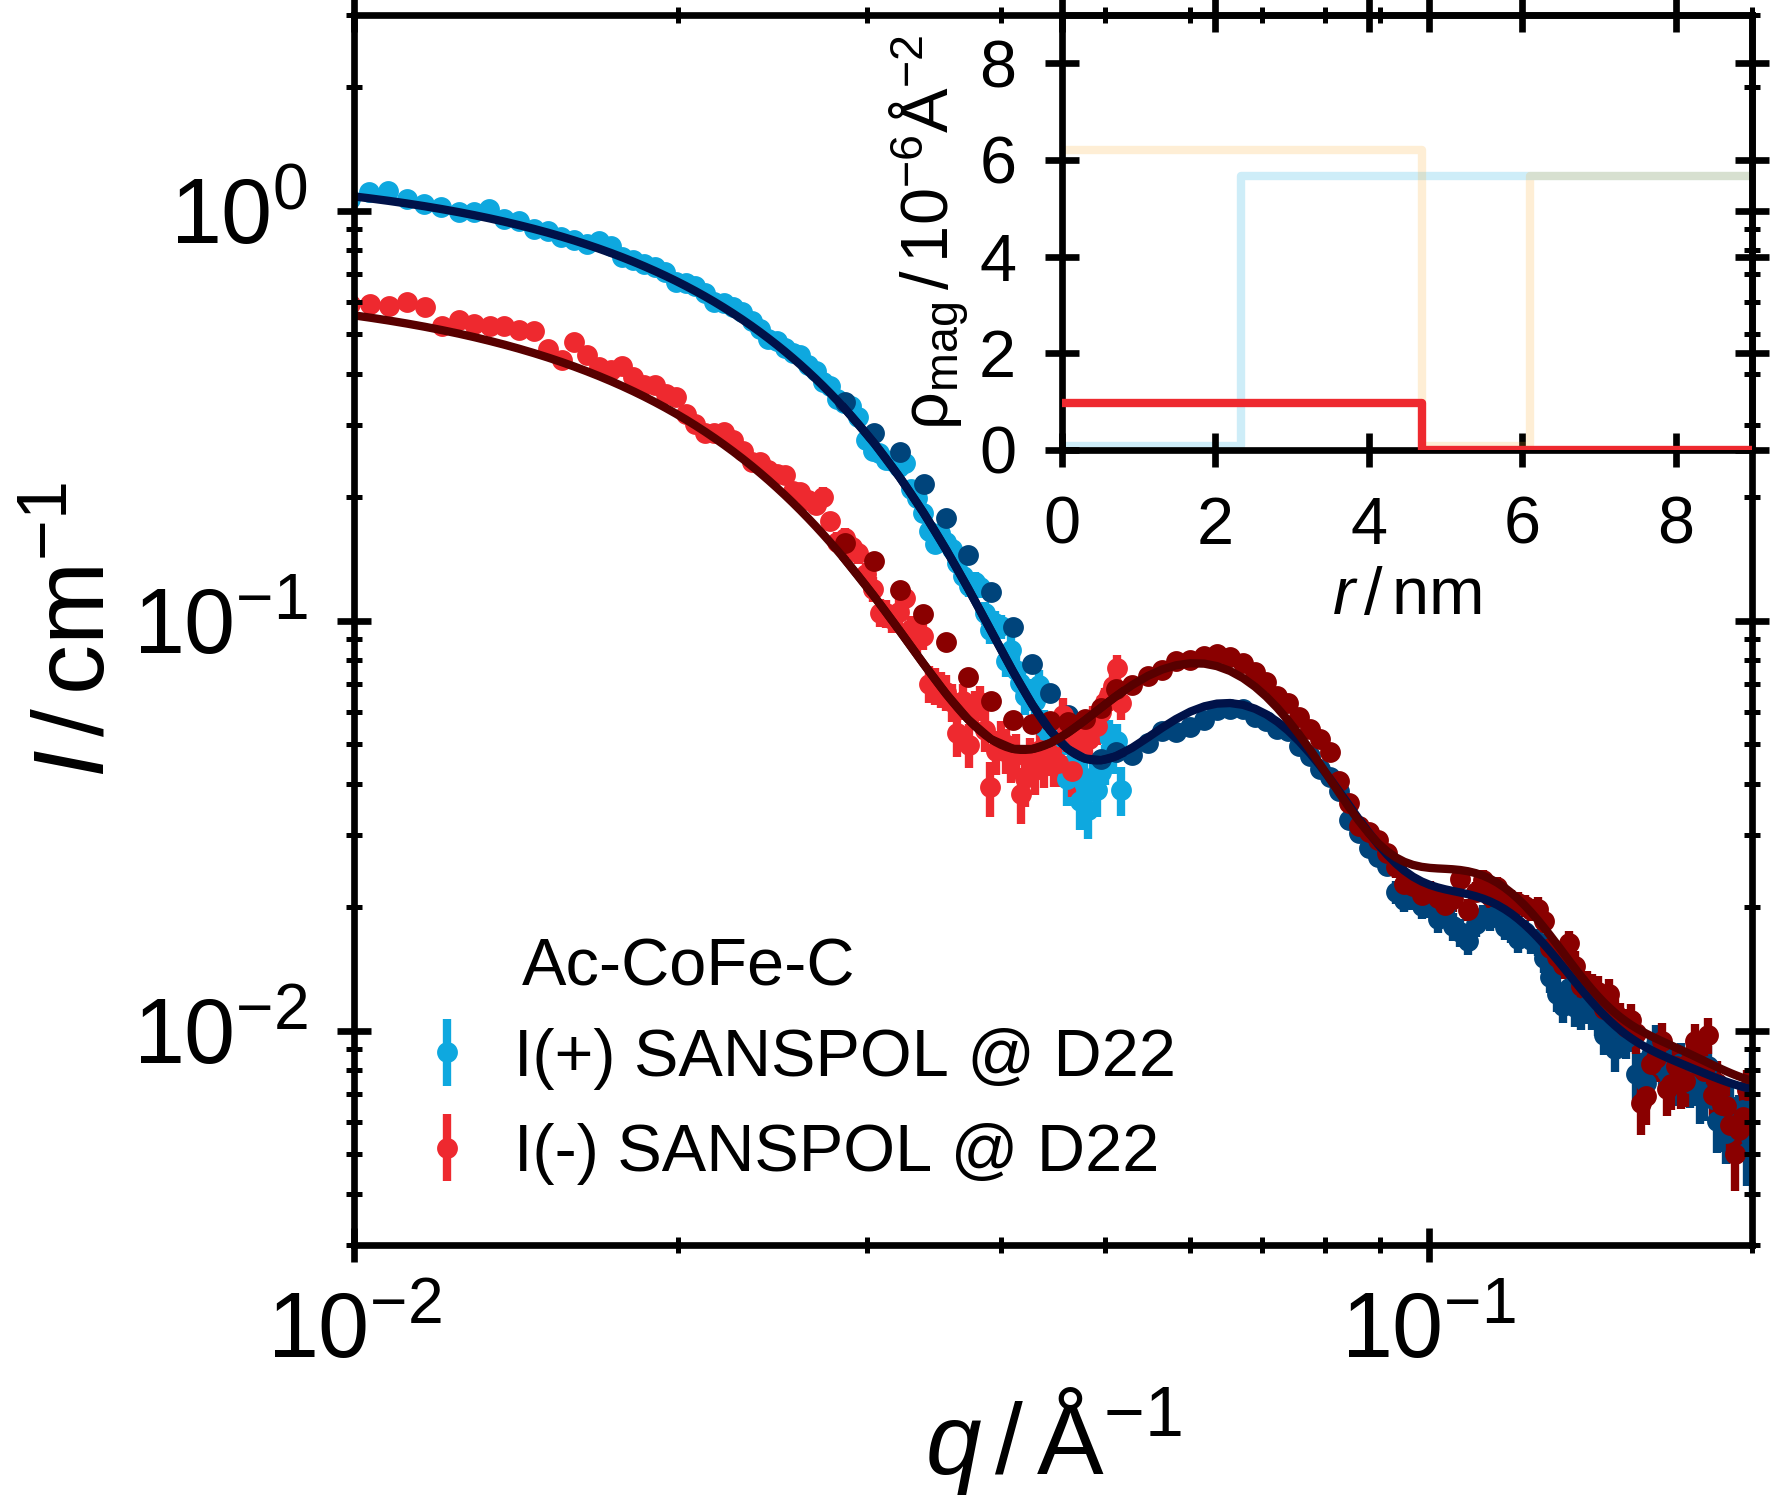
\includegraphics{monolayers_SAS_Ac_CoFe_C_SANSPOLFit}
      \caption{\label{fig:monolayers:nanoparticle:sas:AcOlCoFeC}SAXS and SANS measurement of Ol-CoFe-C (upper left) and Ac-CoFe-C (lower left), as well as SANSPOL at $1.2 \unit{T}$ (right). The data is fit to a superball form factor.}
    \end{figure}

    The surfactant shell thickness are in the range of $1 - 2 \unit{nm}$, which is expected for oleic acid chains.
    As the chains mix with the solvent on the way out, it is expected that the average scattering length density of the shell is not exactly that of bulk oleic acid ($7.8 \cdot 10^{-8} \angstrom^{-2}$), but a mixture with the solvent SLD, which correlates with the model thickness and might explain the reduced value in Ac-CoFe-C.
    The exact thickness, density and shape of the shell is not of detailed interest for the study of the magnetic properties of the nanocubes and therefore in the scope of this work this rough estimate of the shell is good enough for the discussion.

    % SANSPOL <-> VSM at 300K
    The magnetic scattering length density is determined from the SANSPOL data, which is used to determine the magnetization of the nanoparticle using \refeq{eq:looselyPackedNP:nanoparticles:SLDtoMagnetization} to $92(3) \unit{kAm^{-1}}$ for Ol-CoFe-C and $145(2) \unit{kAm^{-1}}$ for Ac-CoFe-C.

    The fitted model is shown in \reffig{fig:monolayers:nanoparticle:sas:AcOlCoFeC} and the important parameter of interest are given in \reftab{tab:monolayers:nanoparticle:sas} for the following discussion, whereas the full set of model parameters is listed in \refapp{ch:appendix:modelparameters:monolayers:sas_olac_cofe_c}.
    \begin{table}[ht]
      \centering
      \caption{\label{tab:monolayers:nanoparticle:sas}Relevant parameters of the superball fit of the small-angle scattering data of the presented nanocubes, the complete set used to describe the models are found in \refapp{ch:appendix:modelparameters:monolayers:sas_olac_cofe_c}.}
      \begin{tabular}{ c | l | l }
          & Ol-CoFe-C & Ac-CoFe-C \\
        \hline
        $R$
          & $5.62(2) \unit{nm}$
          & $4.69(1) \unit{nm}$\\
        $\sigma_R$
          & $9.27(8) \,\%$
          & $11.9(1) \,\%$\\
        $D$
          & $1.63(1) \unit{nm}$
          & $1.16(4) \unit{nm}$\\
        $p$
          & $1.54(3) \unit{nm}$
          & $2.66(9) \unit{nm}$\\
        $\rho_\mathrm{mag}^\mathrm{sans}$
          & $0.268(8) \cdot 10^{-6} \angstrom^{-2}$
          & $0.423(7) \cdot 10^{-6} \angstrom^{-2}$\\
        \hline
        $V_p$
          & $1030(10) \unit{nm^3}$
          & $726(5) \unit{nm}$\\
        $M^\mathrm{sans}$
          & $92(3) \unit{kAm^{-1}}$
          & $145(2) \unit{kAm^{-1}}$\\
        \hline
      \end{tabular}
    \end{table}
    The superball model result confirms the qualitative observation that the Ol-CoFe-C nanoparticles have a smaller size distribution than the Ac-CoFe-C cubes.
    Where the specimen size used to determine size and size distributions in TEM leave the option for a biased result due to possibly missed counting fractions of the dispersion by only measuring a small selected amount of nanoparticles, the large number of particles scanned in the small-angle scattering experiments reveals without bias the average particle size and variation.
    Furthermore, the model gives that on average Ol-CoFe-C has a higher degree of roundness on the corners, visible from the smaller $p$ parameter in comparison to Ac-CoFe-C.
    To see this in imaging experiments, high resolution transmission electron microscopy (HR-TEM) experiments are necessary.
    A study comparing the effectiveness of the superball model in comparison to HR-TEM can be found in \refapp{app:structureCoFe2O4Nanocubes} for three particle batches synthesized similar to Ac-CoFe-C (with a lower heating rate and varied cobalt content, but otherwise same synthesis parameters).

  \paragraphNewLine{Impact of Formfactor on Magnetization Density}

    It's worthwhile to study the impact of the chosen shape model of the nanoparticle on the result of the magnetic scattering density.
    For this purpose, the simpler models of a perfect sphere and cube are fit additionally to the data of Ac-CoFe-C.
    These model provide a good reference point for the parameter values and as the models have one less parameter, they are additionally less prone to systematic errors in the fitting routine due to parameter correlations.
    The result of the cubic and spherical fit are shown in \reffig{fig:monolayers:nanoparticle:sas:SphereCubeFit} with the relevant parameters listed in \reftab{tab:monolayers:nanoparticle:sasSphereCubeFit}.

    \begin{table}[ht]
      \centering
      \caption{\label{tab:monolayers:nanoparticle:sasSphereCubeFit}Relevant parameters of the sphere and cube fit to the small-angle scattering data of Ac-CoFe-C, the complete set of parameters is found in \refapp{ch:appendix:modelparameters:monolayers:sas_olac_cofe_c}.}
      \begin{tabular}{ c | l | l }
          & Sphere & Cube \\
        \hline
        $R, \, a$
          & $5.56(2) \unit{nm}$
          & $9.01(2) \unit{nm}$\\
        $\sigma_R, \, \sigma_a$
          & $13.0(3) \,\%$
          & $10.7(2) \,\%$\\
        $D$
          & $1.46(4) \unit{nm}$
          & $1.03(4) \unit{nm}$\\
        $\rho_\mathrm{mag}^\mathrm{sans}$
          & $0.502(8) \cdot 10^{-6} \angstrom^{-2}$
          & $0.429(7) \cdot 10^{-6} \angstrom^{-2}$\\
        \hline
        $V_p$
          & $720(4) \unit{nm^{3}}$
          & $731(3) \unit{nm^{3}}$\\
        $M^\mathrm{sans}$
          & $172(3) \unit{kAm^{-1}}$
          & $147(2) \unit{kAm^{-1}}$\\
        \hline
      \end{tabular}
    \end{table}

    It's clearly visible by looking at the SAXS data that the spherical model underestimates the intensity of the first order peak, while the cube model overestimates it, whereas the superball was able to adjust in between.
    The determined particle volume varies only weakly from the specific choice of the model and therefore the model has only a minor effect on the rescaling procedure that is applied to the vibrating sample magnetometry data.
    From SANSPOL, it is visible that parameters such as the shell thickness, particle magnetization, as well as the particle concentration (listed in complete parameter set in \refapp{ch:appendix:modelparameters:monolayers:sas_olac_cofe_c}), are stronger affected by the choice of model in the fitting process.
    This becomes especially visible in the observation that the cube model estimates a smaller shell thickness and magnetization, whereas the sphere model suggests values that are a magnitude of $30 - 50 \unit{\%}$ higher.

    \begin{figure}[tb]
      \centering
      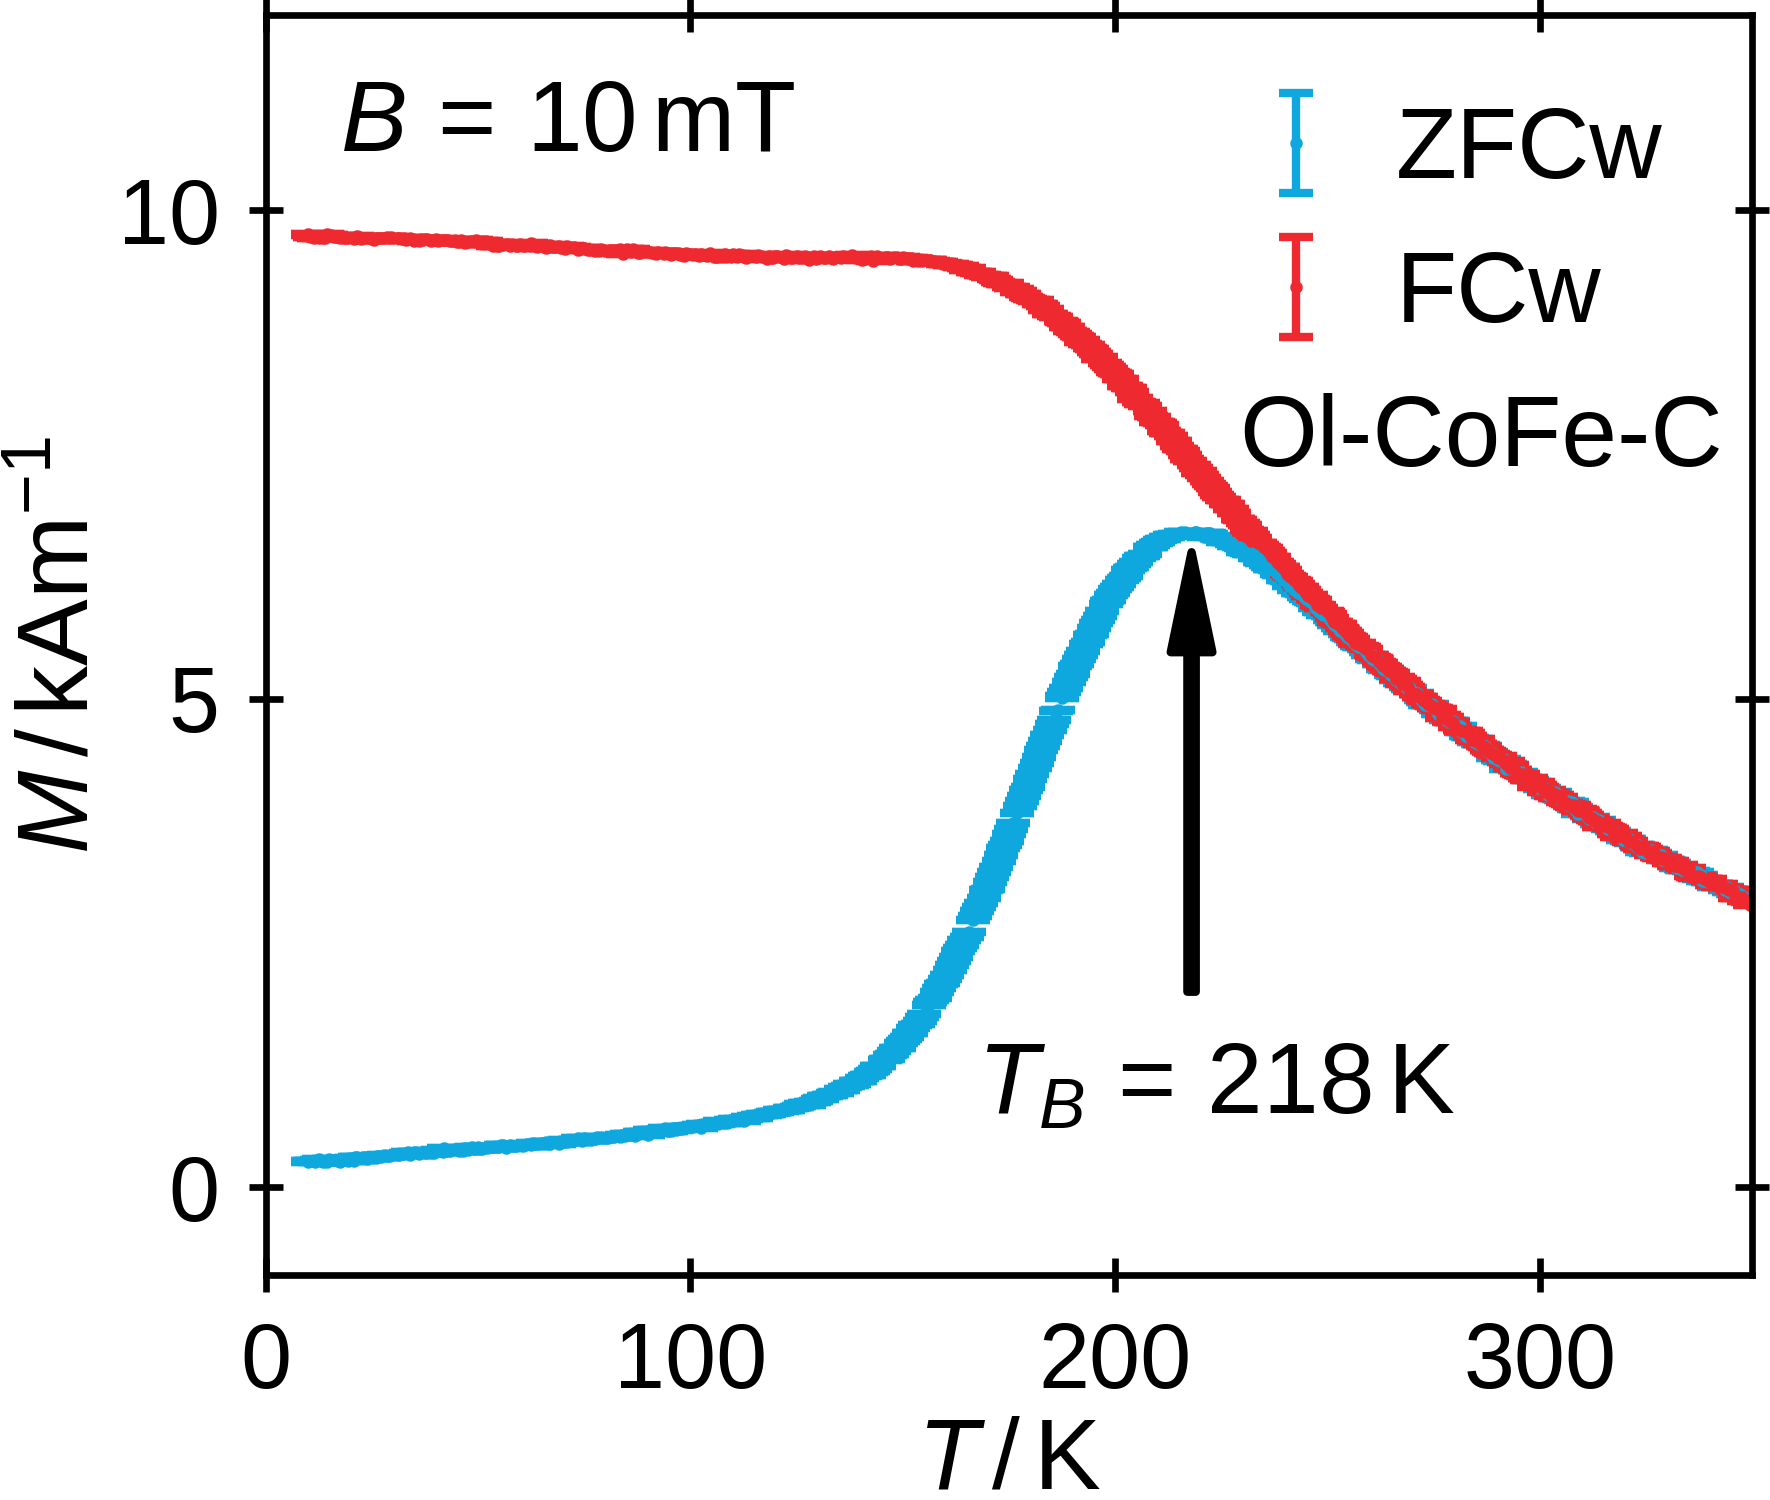
\includegraphics{monolayer_PPMS_ZFC_FC_ML_Ol_CoFe_C}
      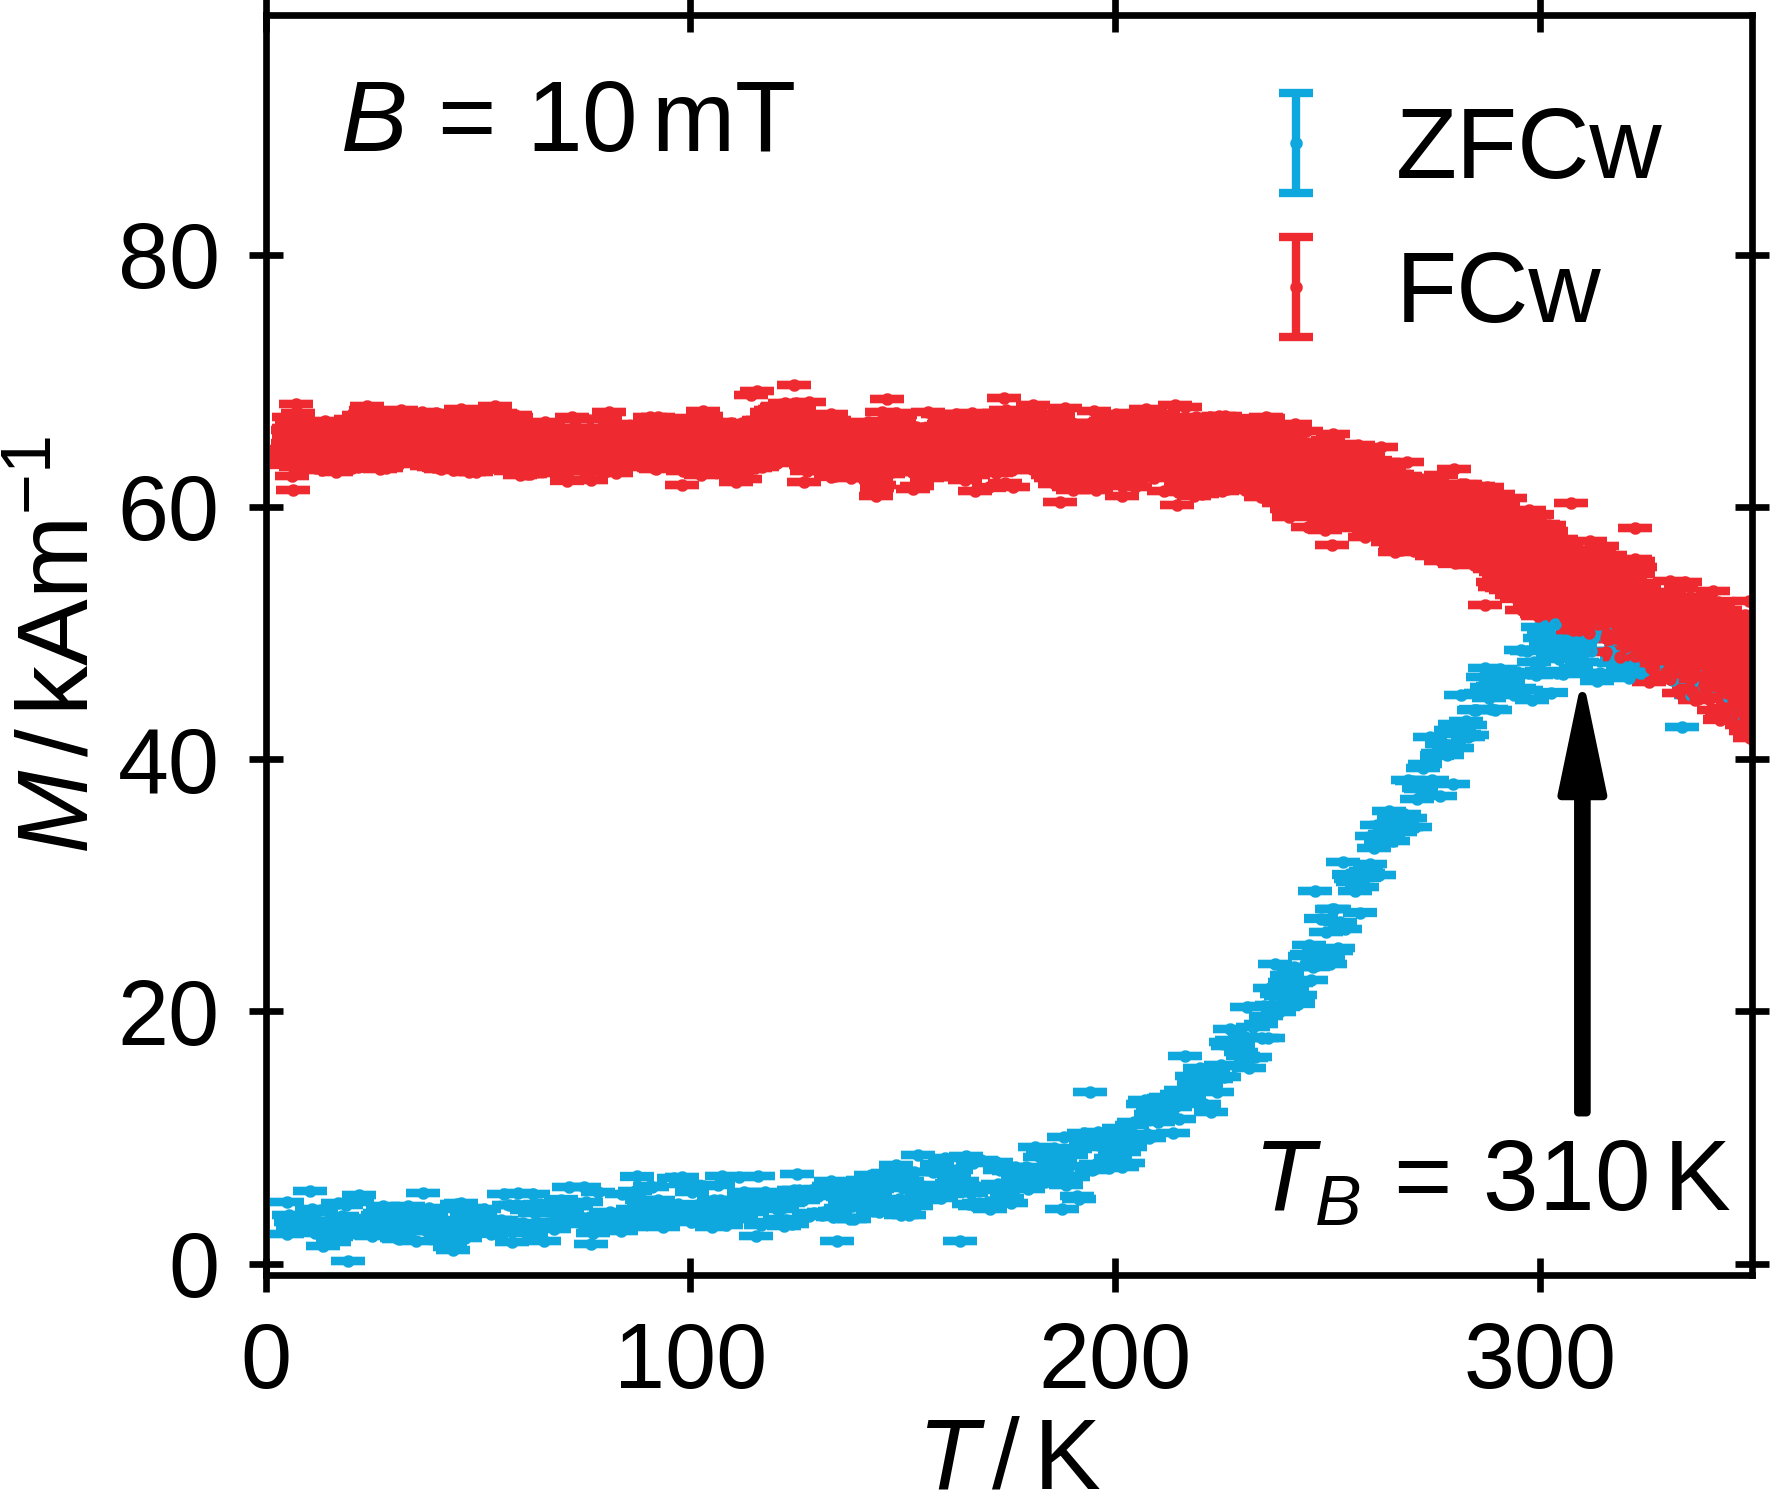
\includegraphics{monolayer_PPMS_ZFC_FC_ML_Ac_CoFe_C}
      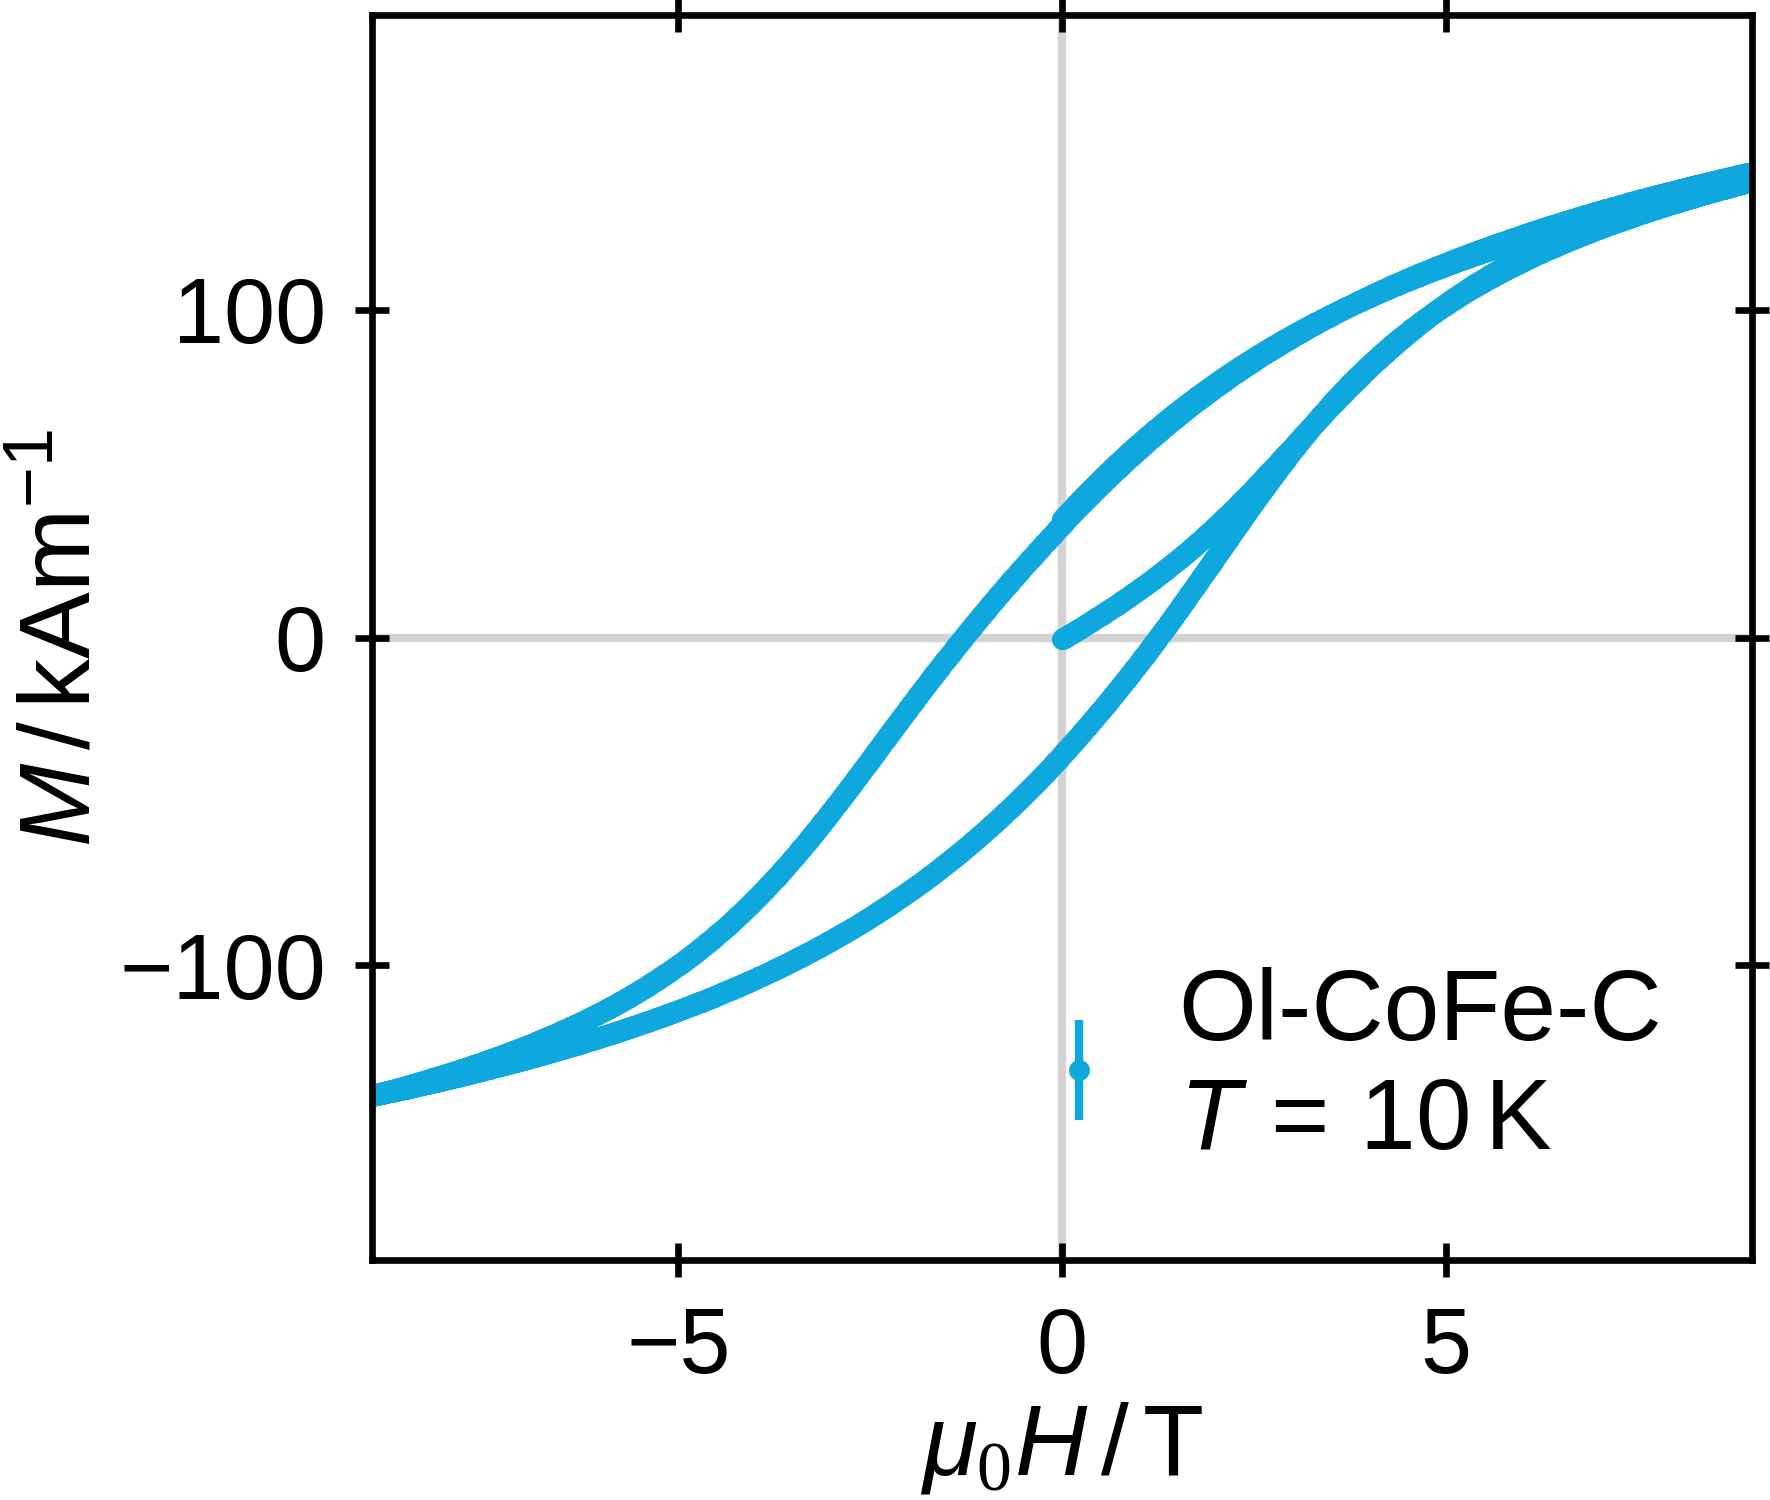
\includegraphics{monolayer_VSM_10K_Ol_CoFe_C}
      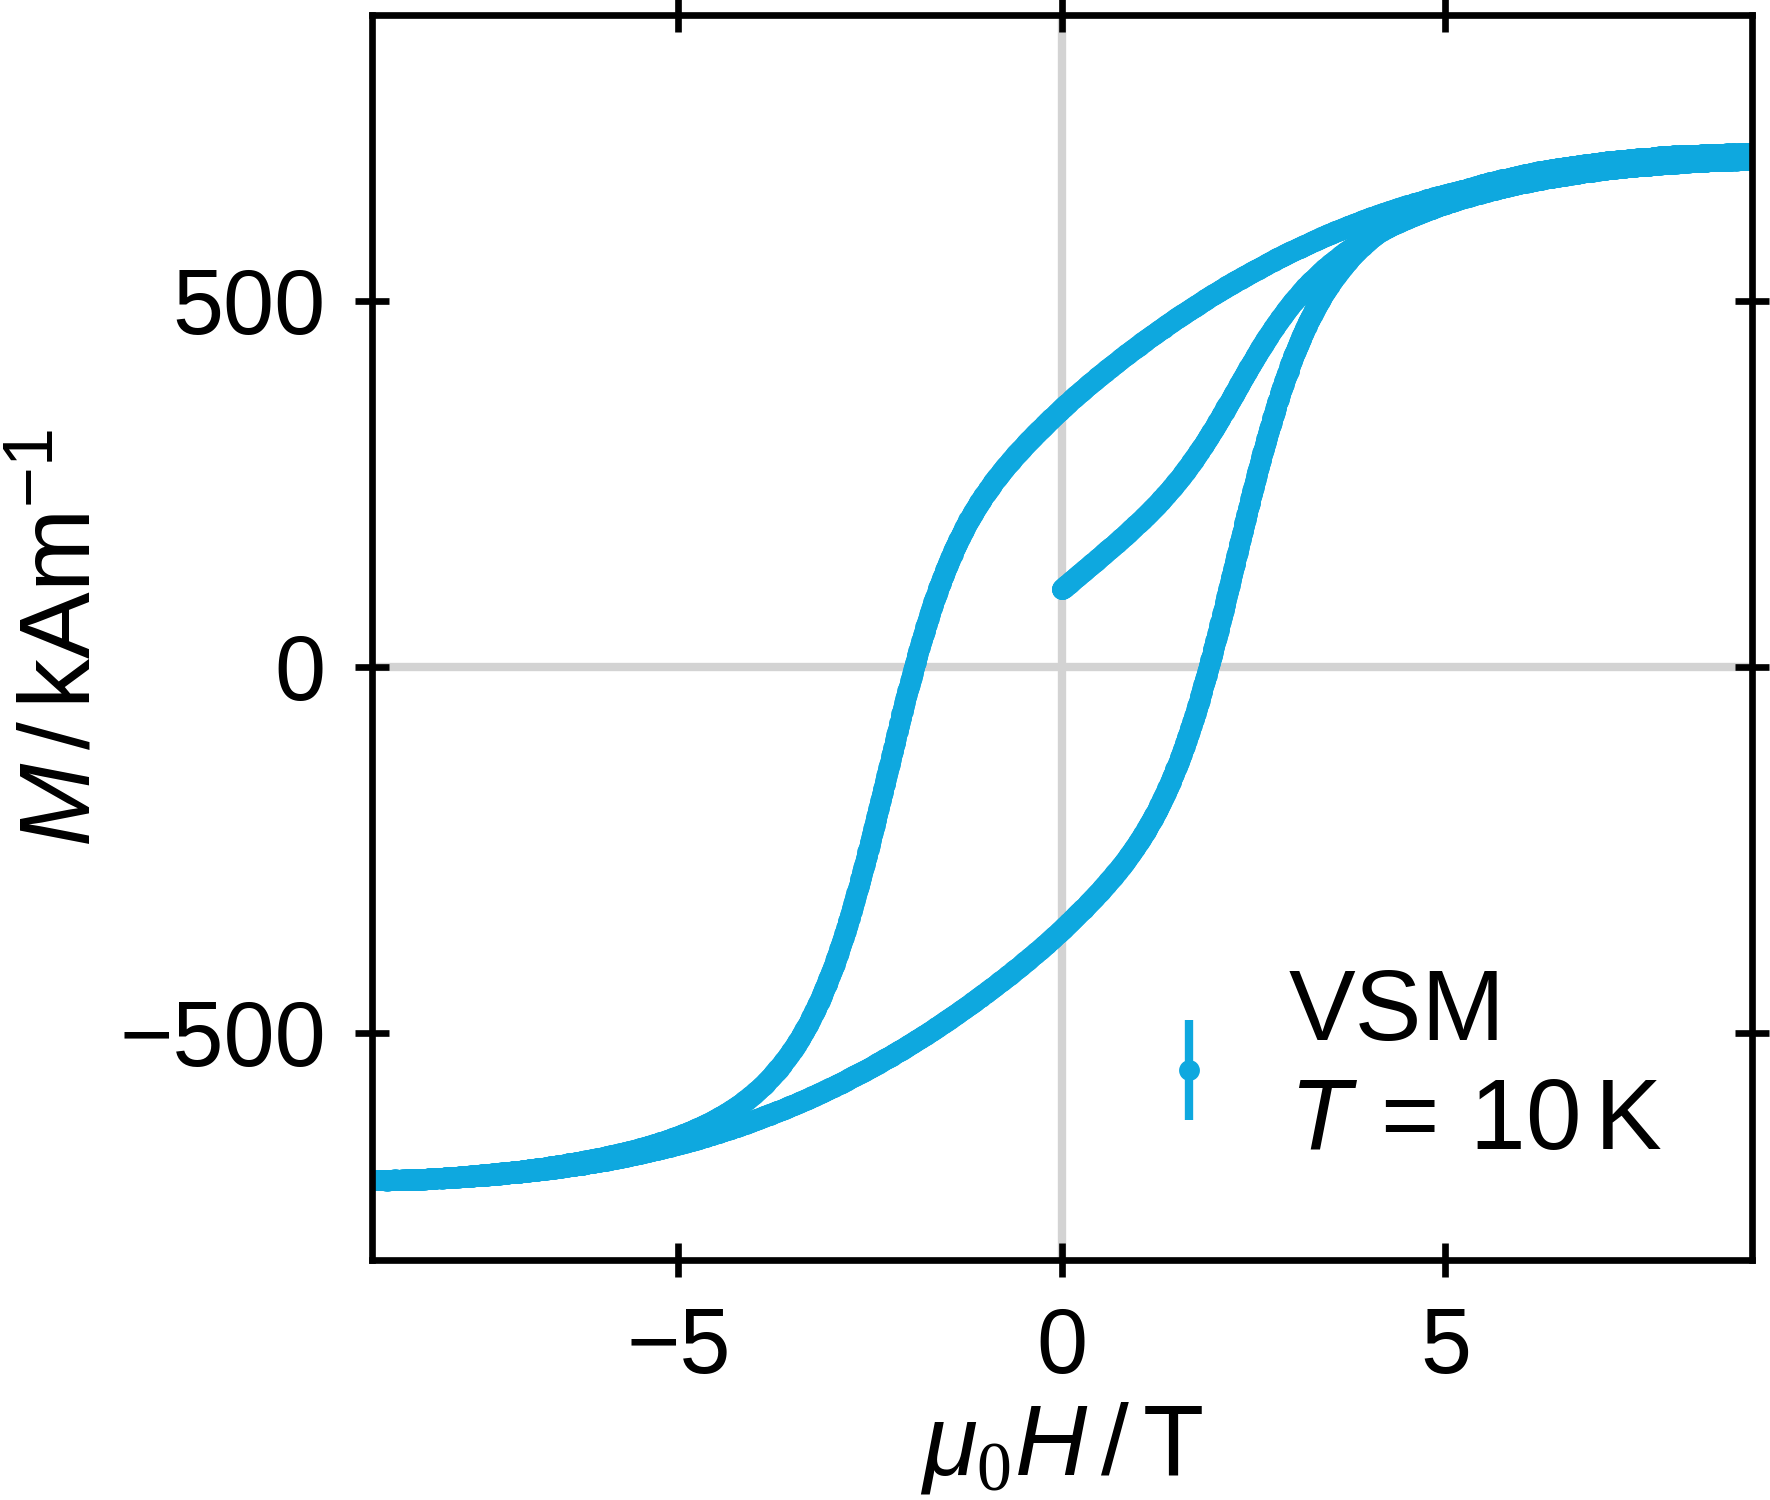
\includegraphics{monolayer_VSM_10K_Ac_CoFe_C}
      \caption{\label{fig:monolaye rs:nanoparticle:vsm10K}Low temperature hysteresis measurement of frozen Ol-CoFe-C (left) and Ac-CoFe-C (right) using the same samples as in \reffig{fig:monolayers:nanoparticle:vsm}.}
    \end{figure}

    \begin{figure}[tb]
      \centering
      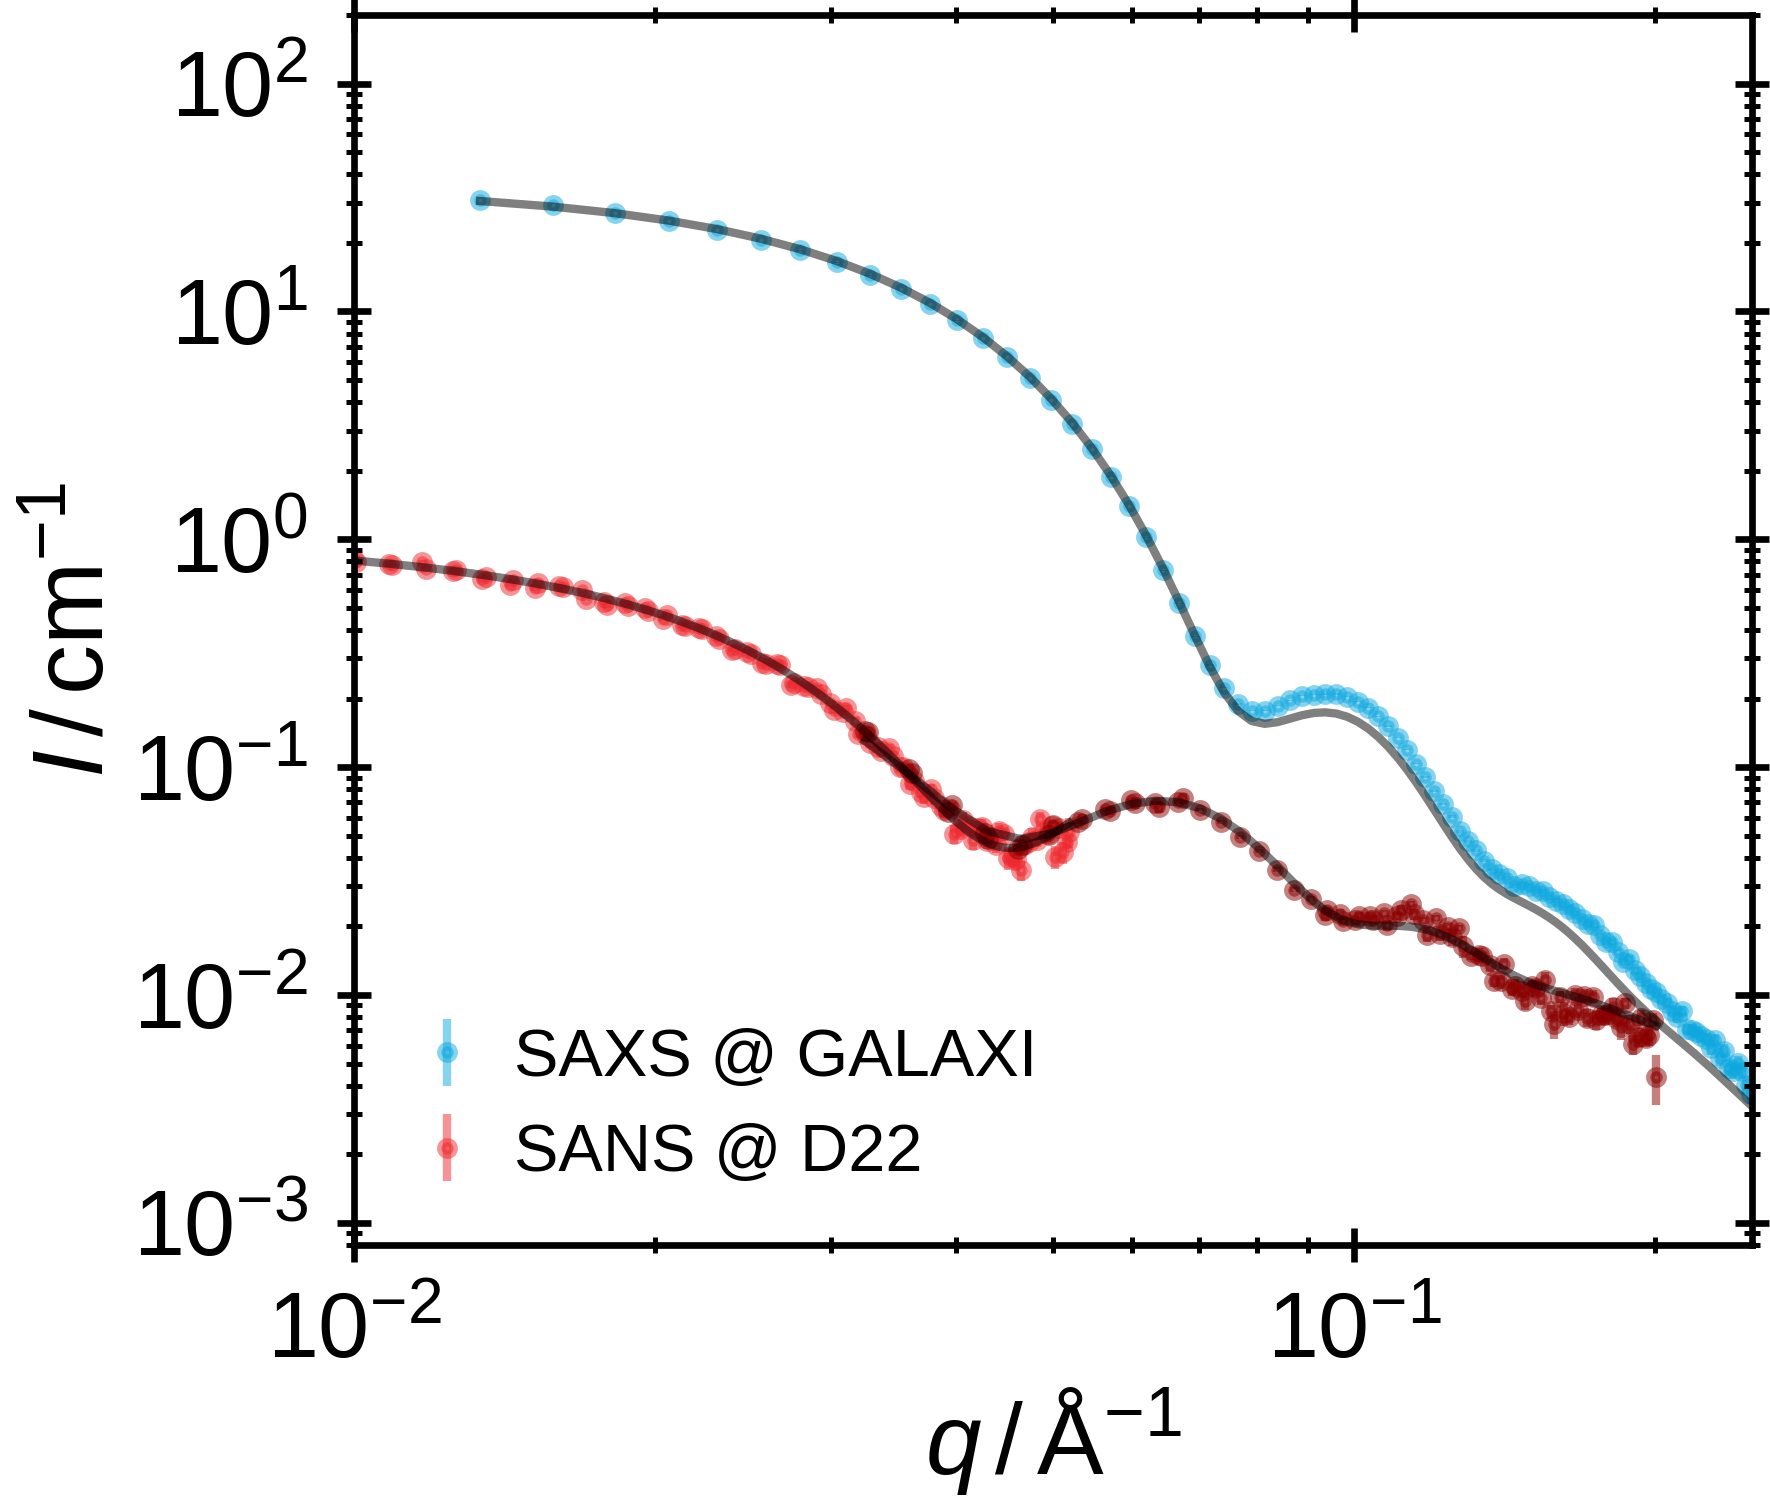
\includegraphics{monolayers_SAS_Ac_CoFe_C_SASSphereModelFit}
      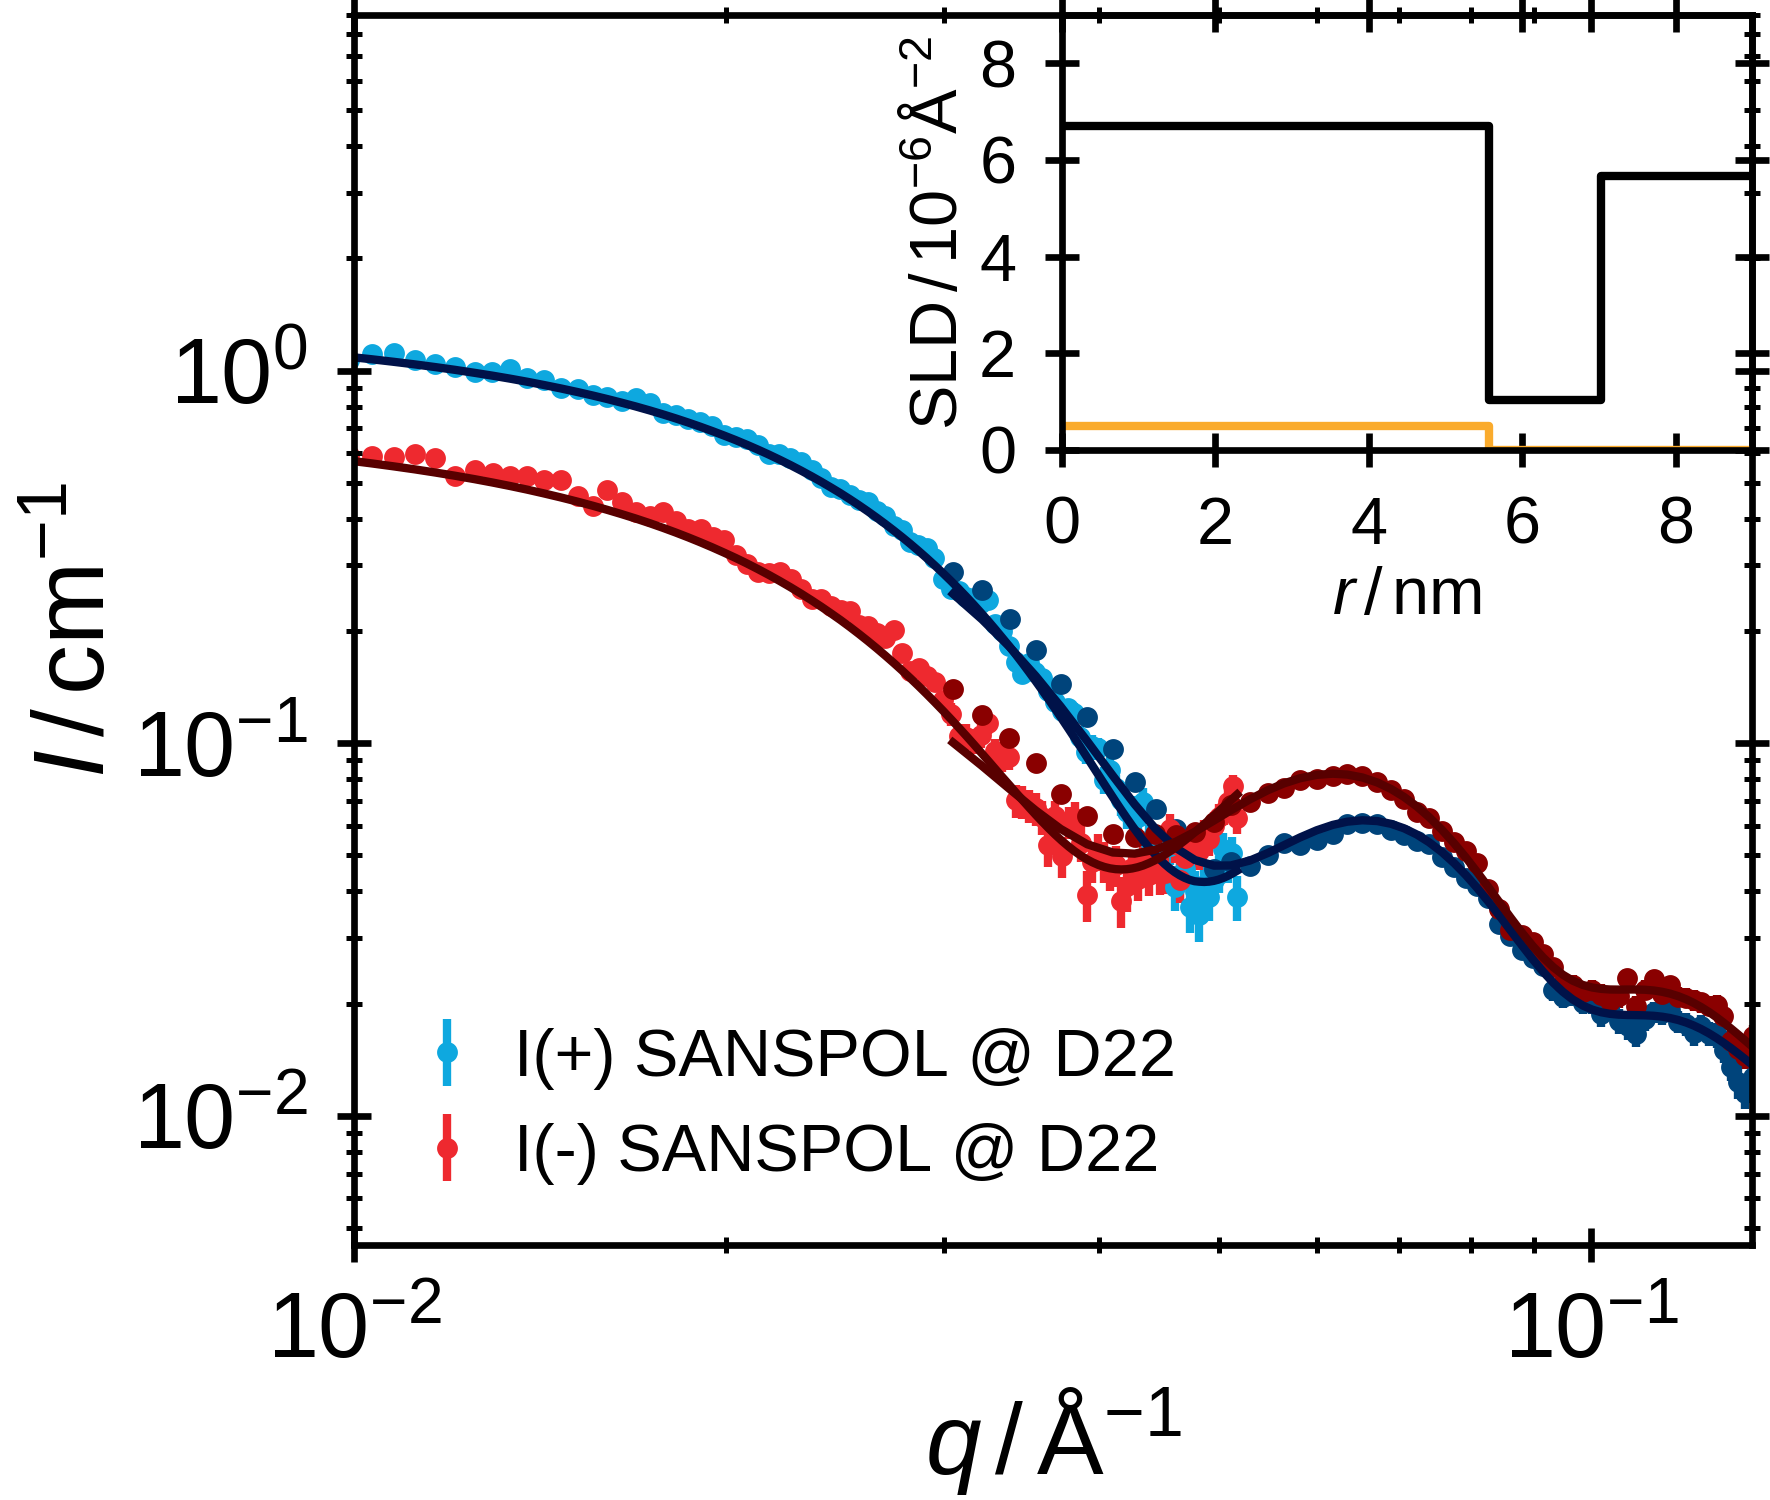
\includegraphics{monolayers_SAS_Ac_CoFe_C_SANSPOLSphereModelFit}
      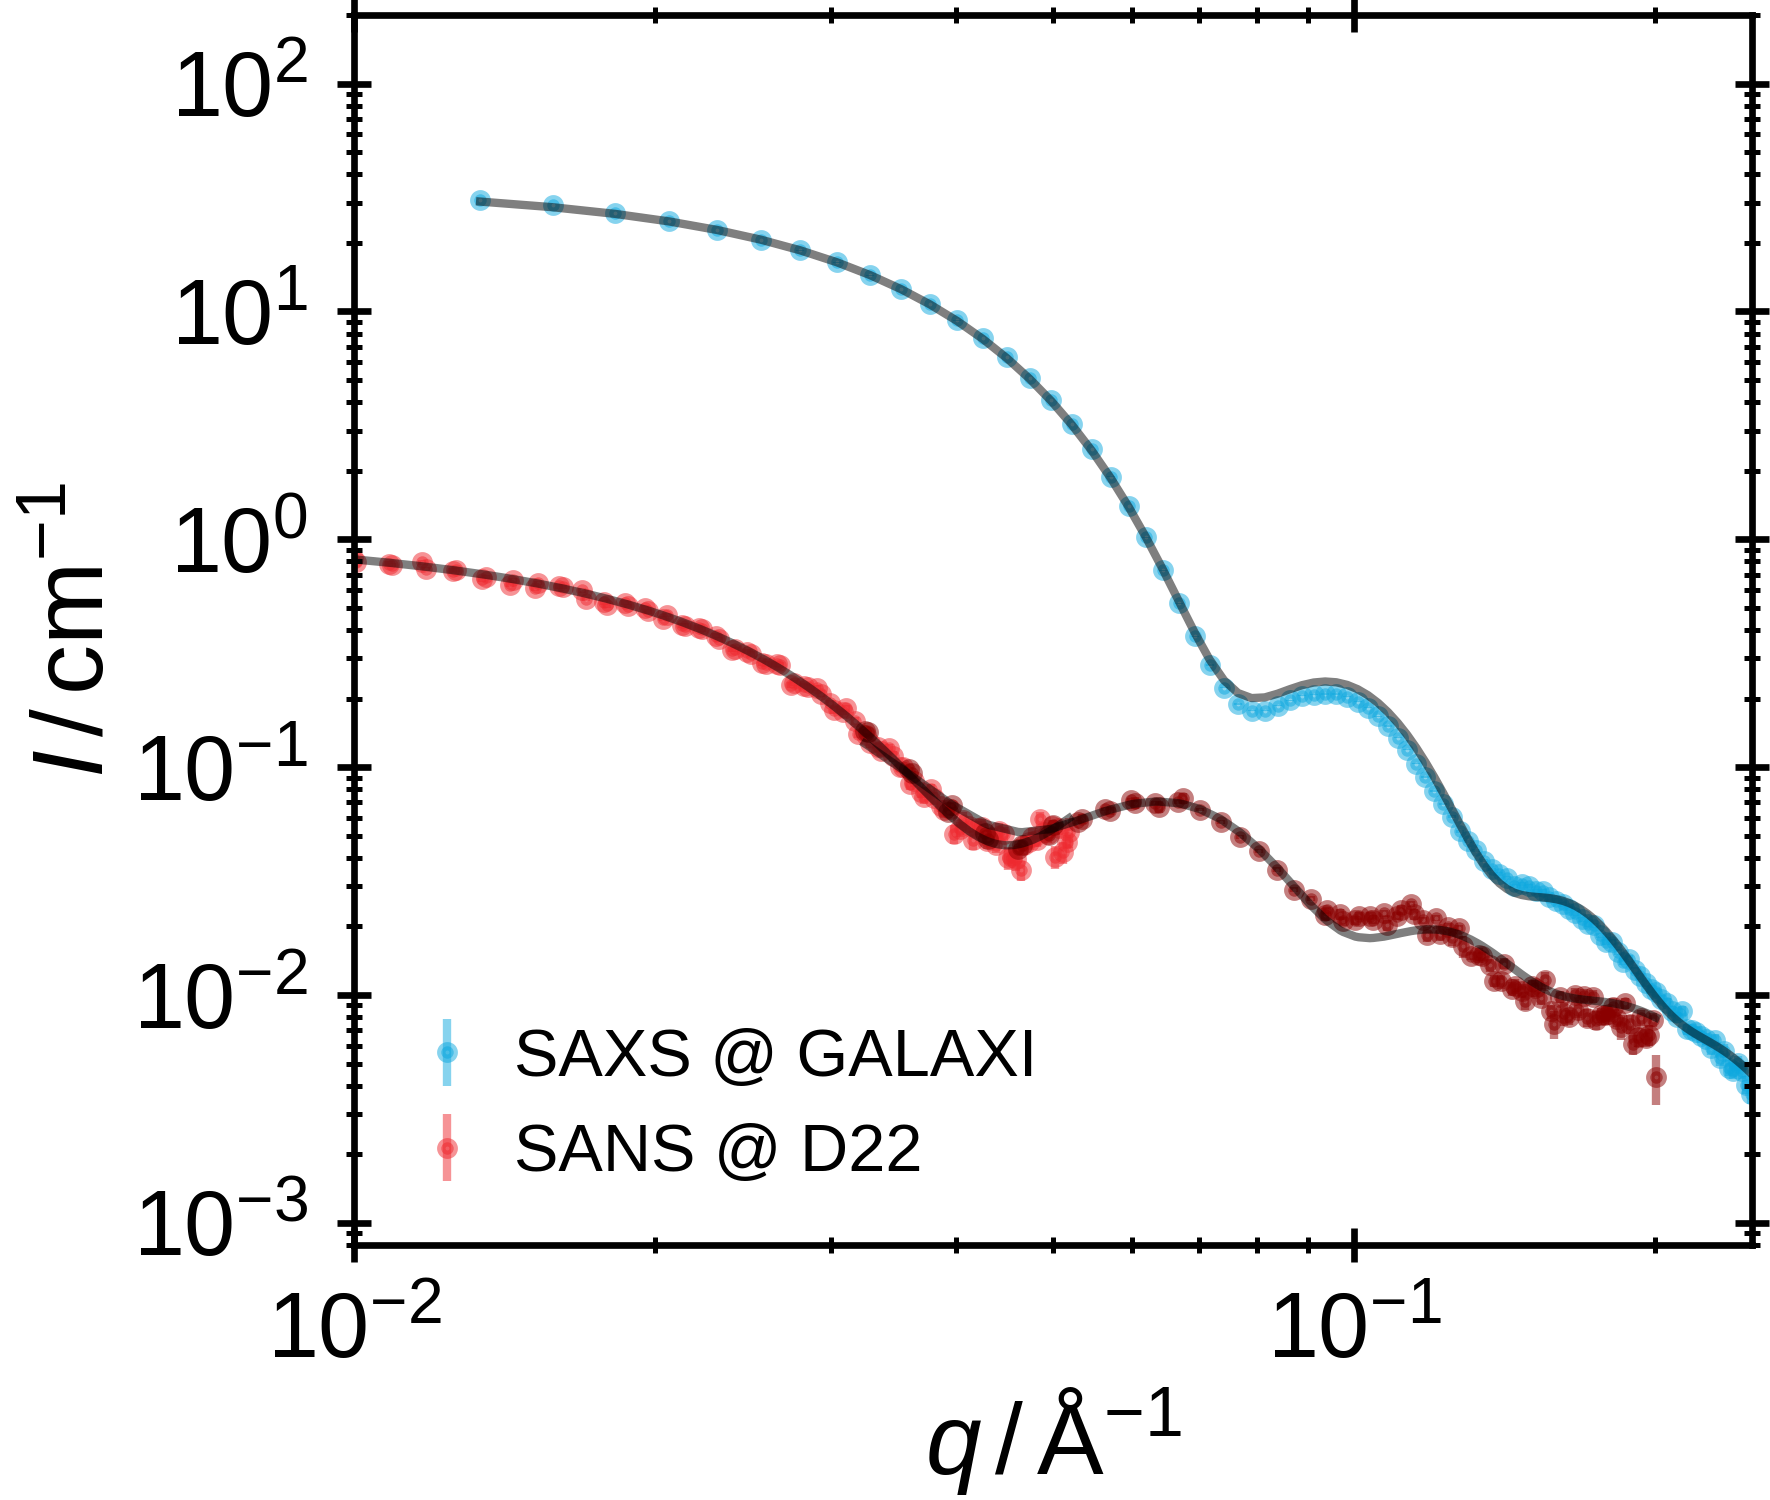
\includegraphics{monolayers_SAS_Ac_CoFe_C_SASCubeModelFit}
      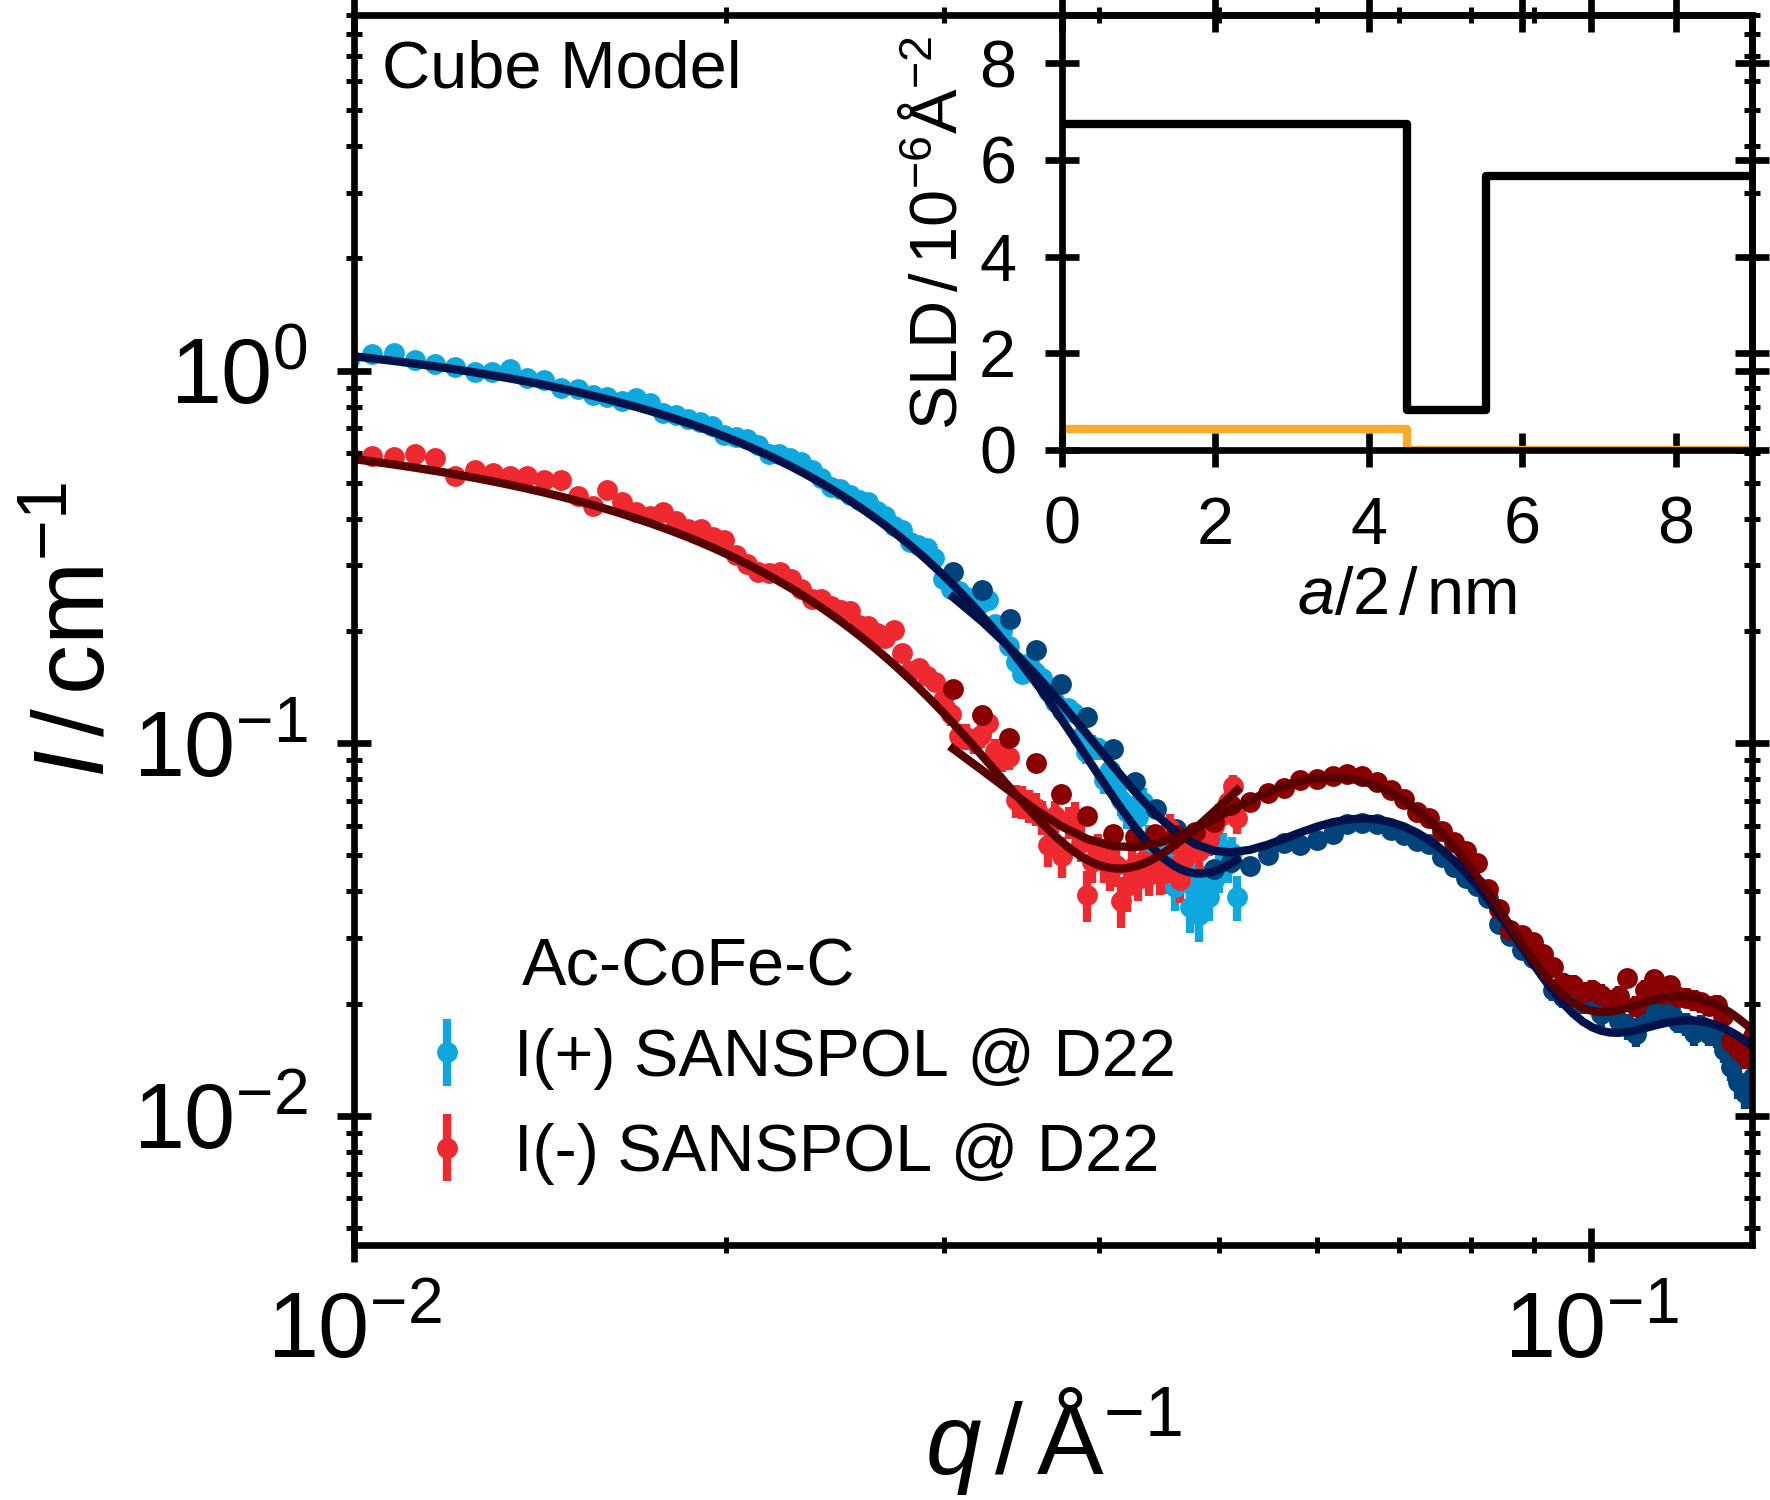
\includegraphics{monolayers_SAS_Ac_CoFe_C_SANSPOLCubeModelFit}
      \caption{\label{fig:monolayers:nanoparticle:sas:SphereCubeFit}Best sphere (upper) and cube model (lower) fit to the same SAS data of Ac-CoFe-C fitted in \reffig{fig:monolayers:nanoparticle:sas:AcOlCoFeC}. The left images show the fit of the nuclear structure for the two models, and the right the determination of the magnetic structure.}
    \end{figure}
\end{document}